\begin{figure}[H]
		\centering
(A)\\
	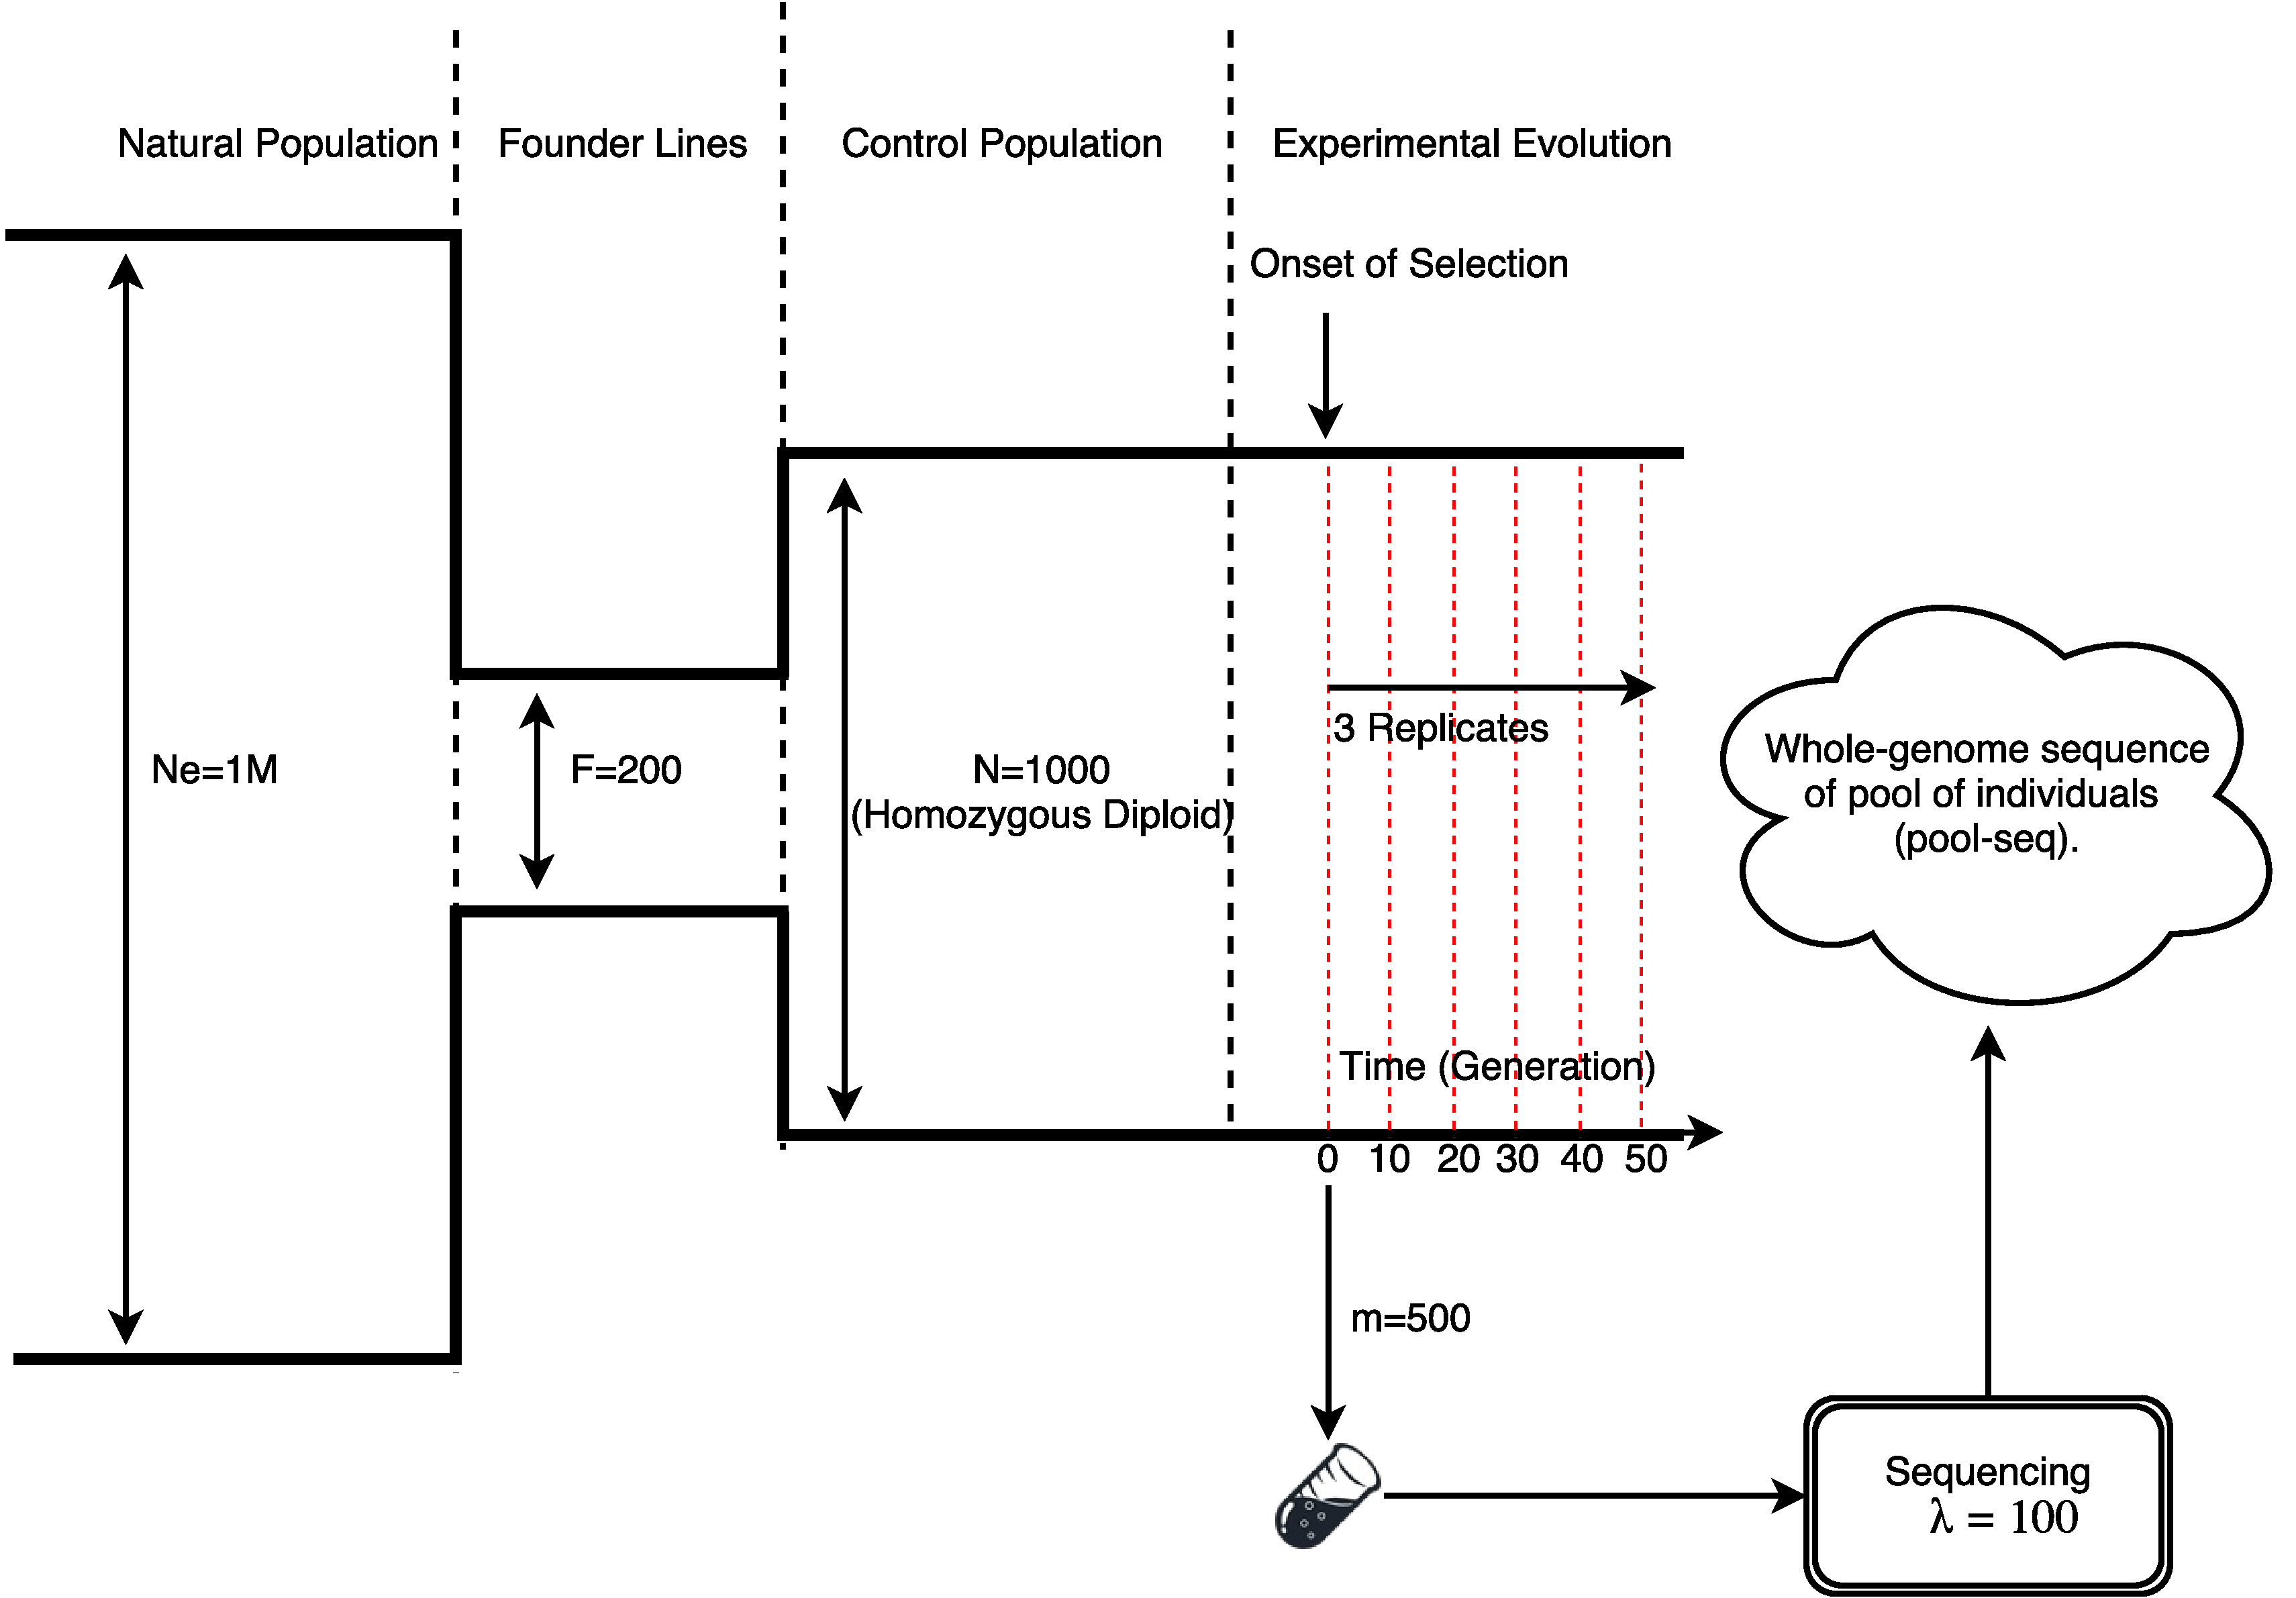
\includegraphics[trim=0in 0in .2in 0.02in , 
	clip,width=0.7\textwidth]{ExperimentalEvolution.pdf}\\

\begin{tabular}{l|l}
		\hline\\
		(B) &(C)\\
		\raisebox{0.1in}{
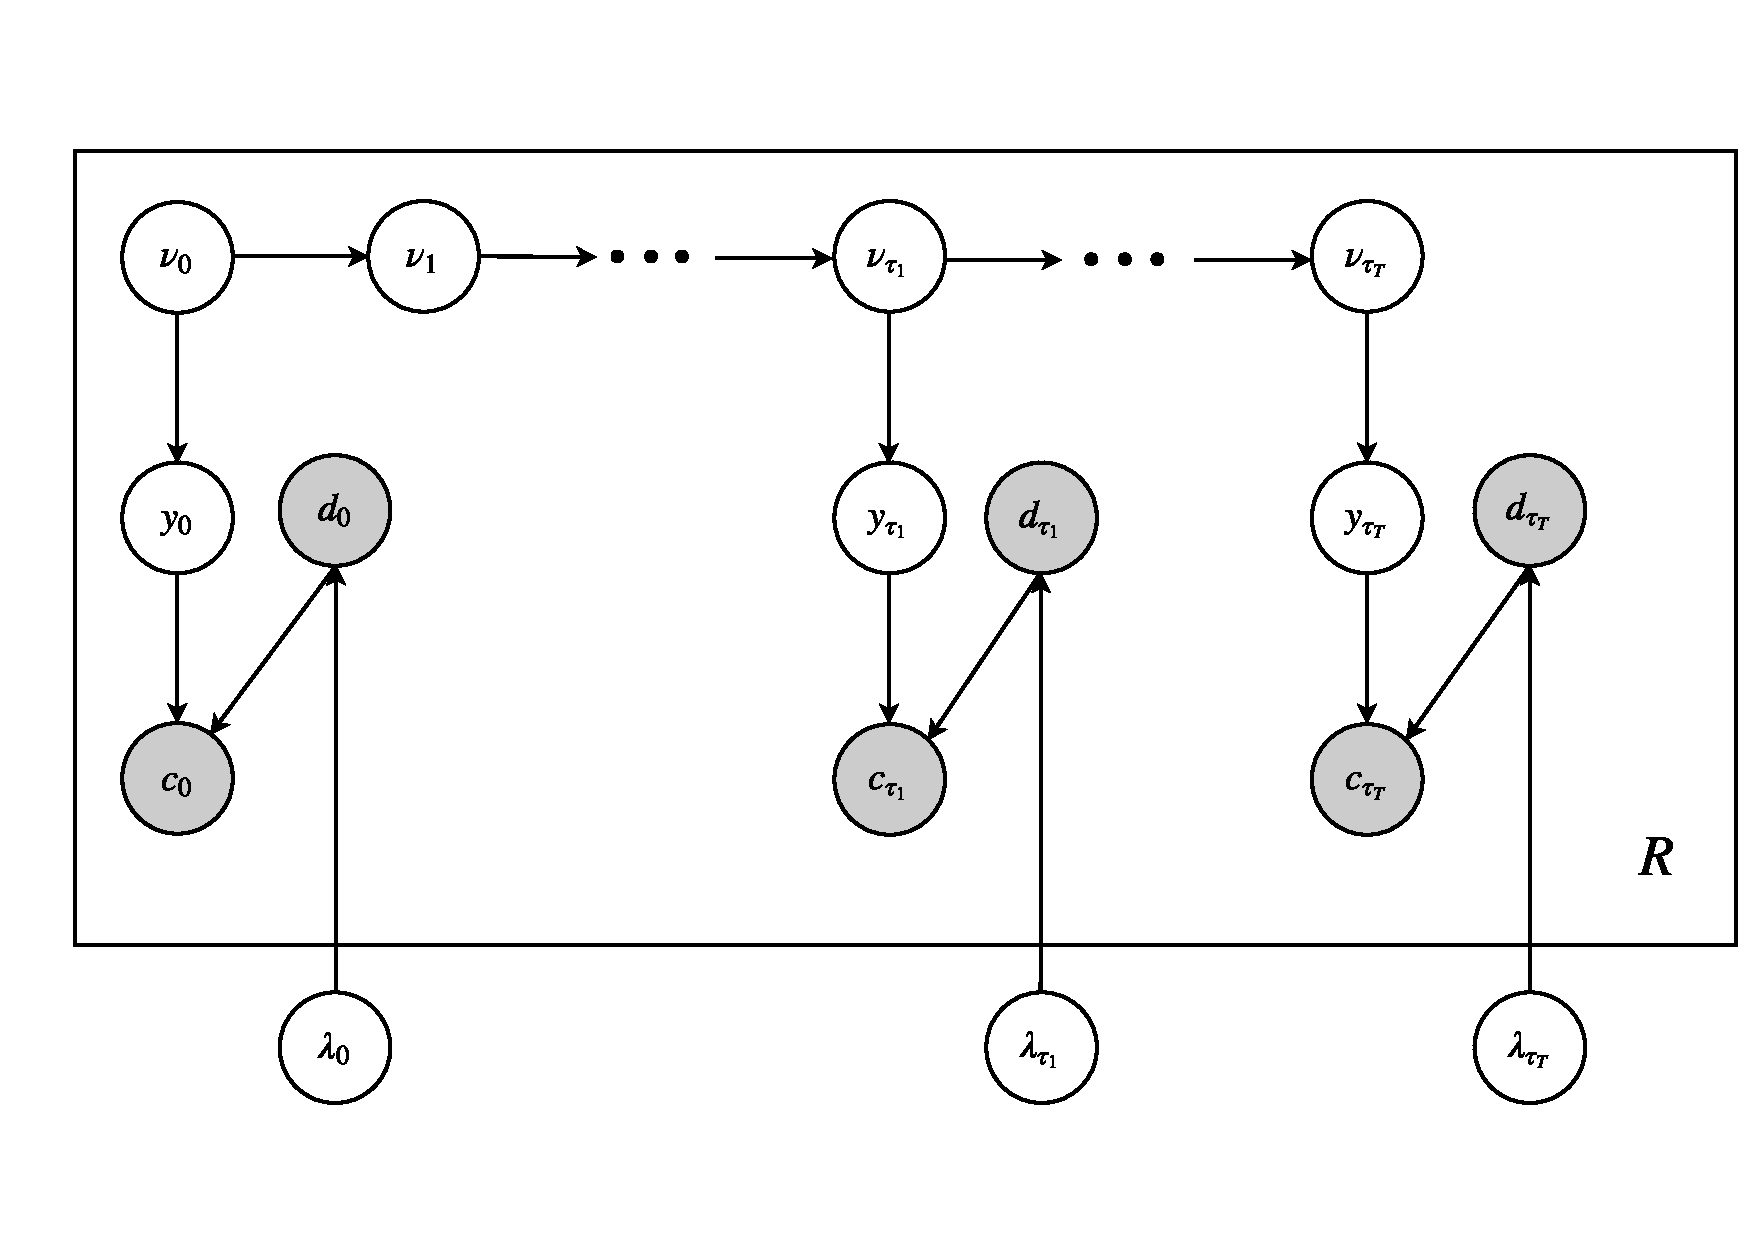
\includegraphics[trim=0in 0.in 0in 
0.0in,clip,width=0.45\textwidth]{HMMGM.pdf}}
& 	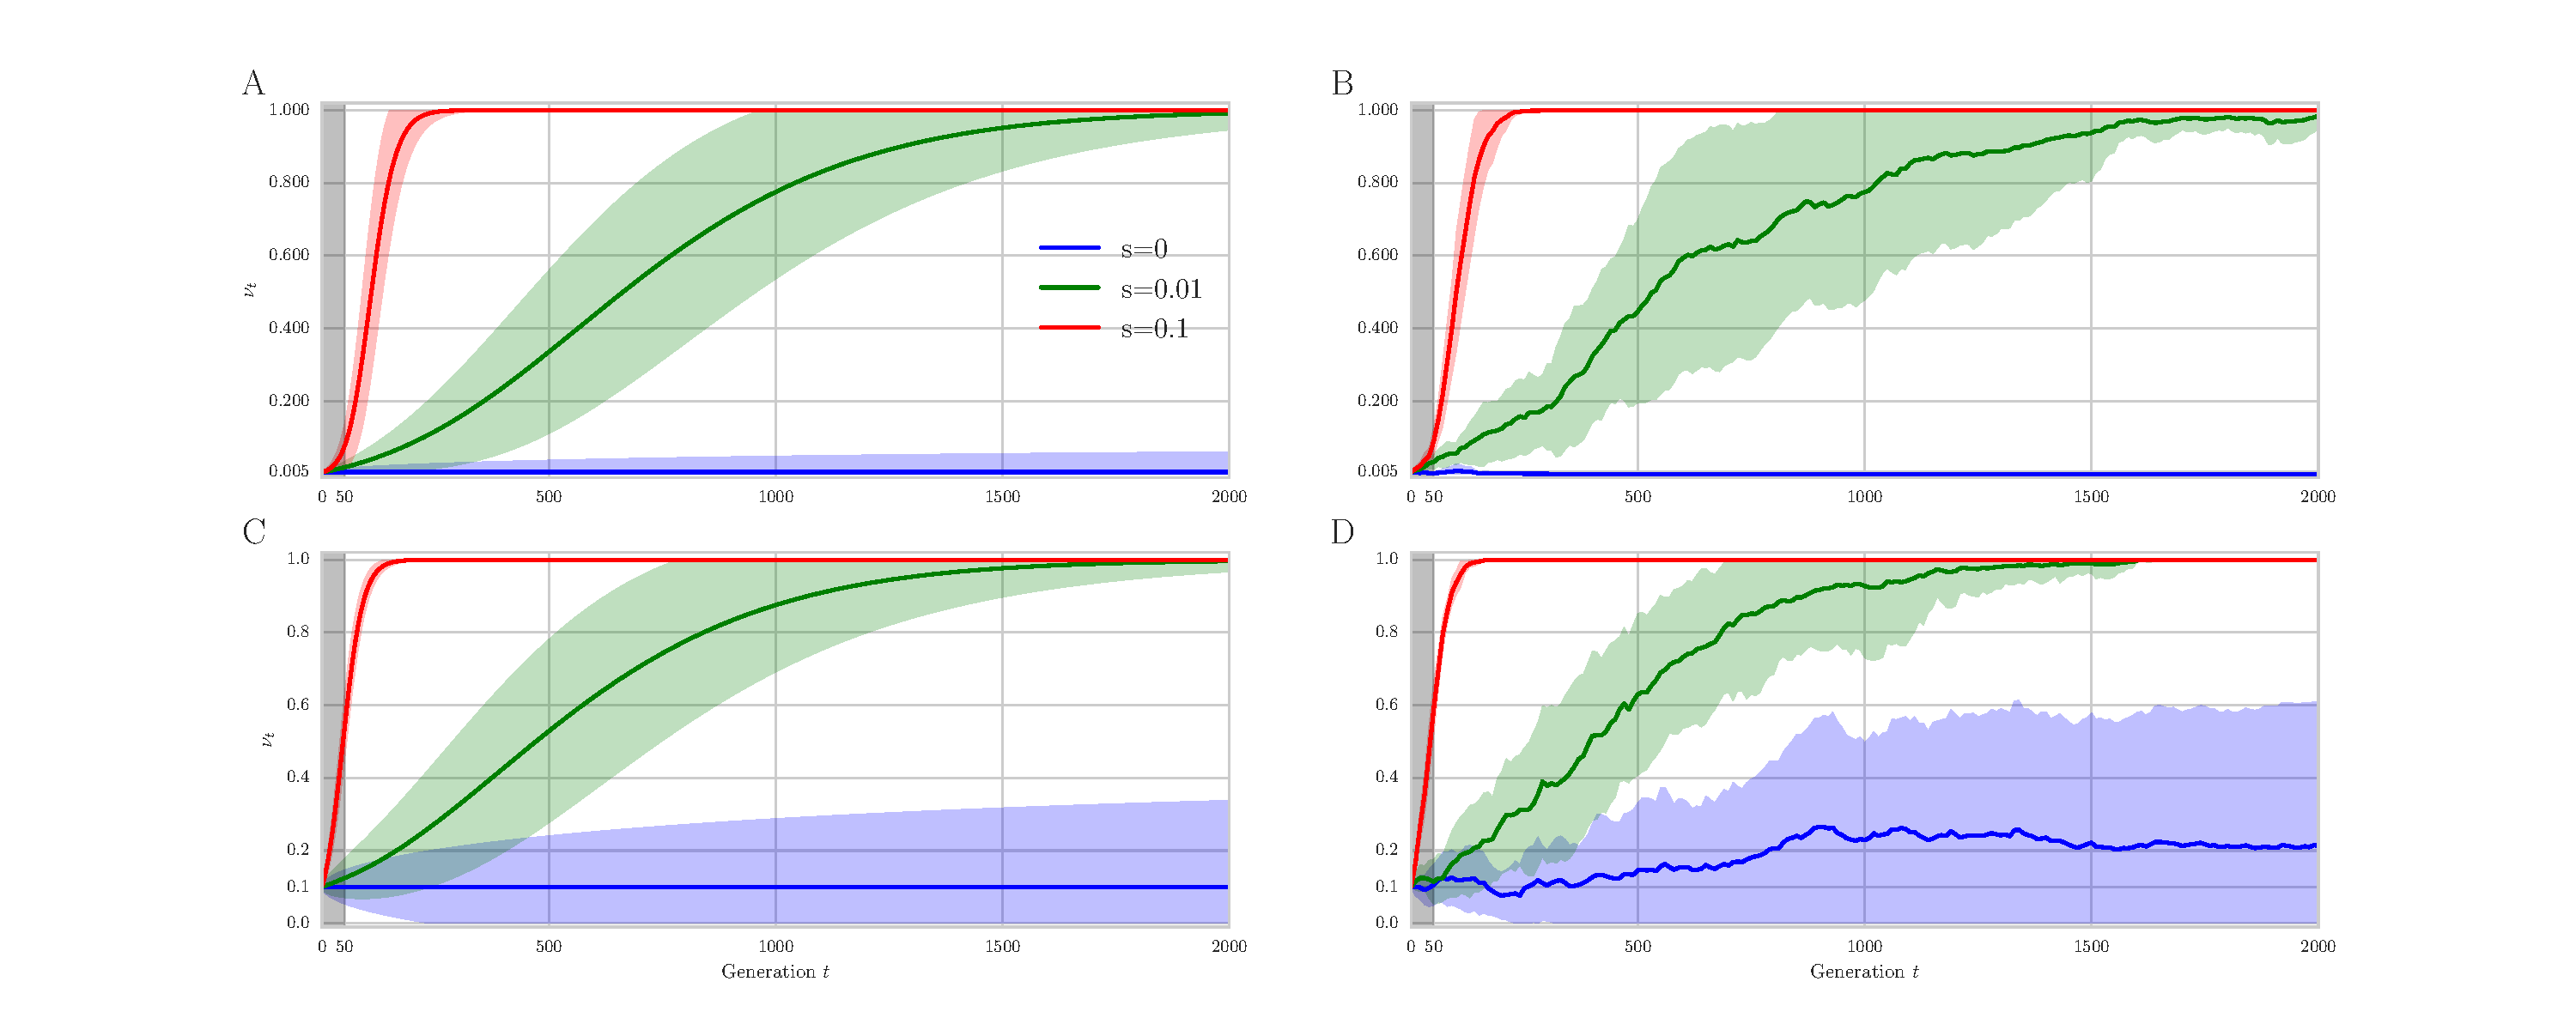
\includegraphics[trim=0in 0.in 0in 
0.0in,clip,width=0.45\textwidth]{AF.pdf}	

\end{tabular}
\hspace{-1in}
\caption{{\bf Evolve and Resequence Selection Experiments on \dmel.}
  (A) Typical configuration in which time-series data is collected for
  \dmel. A small set of founder lines ($F=200$) is selected from a
  large population ($N_o=10^{6}$), and used to create a sub-population
  of isofemale lines. Multiple replicates of the population are
  evolved and resequenced to collect time-series genomic data. For
  sequencing, $n$ individuals are randomly sampled and sequenced with
  coverage $\lambda$.  (B) Graphical model showing dependence of the
  random variables in the single-locus model used to compute \comale\
  statistics. Observed variables, $c$ (derived allele read count) and
  $d$ (total read count) are shaded. The variables $\nu,y,\lambda$
  denote allele frequency, sampled allele frequency, and mean
  sequencing coverage, respectively. (C) Mean and 95\% confidence
  interval of the theoretical (i,iii) and empirical (ii,iv)
  trajectories of the favored allele for hard (i,ii) and soft (iii,iv)
  sweep scenarios and $N=1000$.  The first $50$ generations are shaded
  in gray to represent the sampling span of sampling in short-term
  experiments, illustrating the difficulty in predicting selection at
  early stages of selective sweep.  }
\label{fig:1}
\end{figure}



\begin{figure}[H]
	\centering
	\includegraphics[width=\textwidth]{{markovDists}.pdf}
        \caption{{\bf Comparison of empirical distributions of allele
            frequencies (red) versus predictions from Brownian
            Motion (green), and Markov chain (blue).}\\
          Comparison of empirical and theoretical distributions under
          neutral evolution (panels A-F) and selection (panels G-M)
          with different starting frequencies $\nu_0\in\{0.005,0.1\}$
          and sampling times of $\Tc=\{0,\tau\}$, where $\tau \in
          \{1,10,100\}$ and $N=1000	$.  For each panel, the empirical 
          distribution
          was computed over 100,000 simulations.  Brownian motion
          (Gaussian approximation) provides poor approximations when
          initial frequency is far from 0.5 (A) or sampling is sparse
          (B,C,E,F). In addition, Brownian motion can only provide
          approximations under neutral evolution. In contrast, Markov
          chain consistently provides a good approximation in all
          cases.}
	\label{fig:markov}
\end{figure}

\begin{figure}[H]
	\centering
	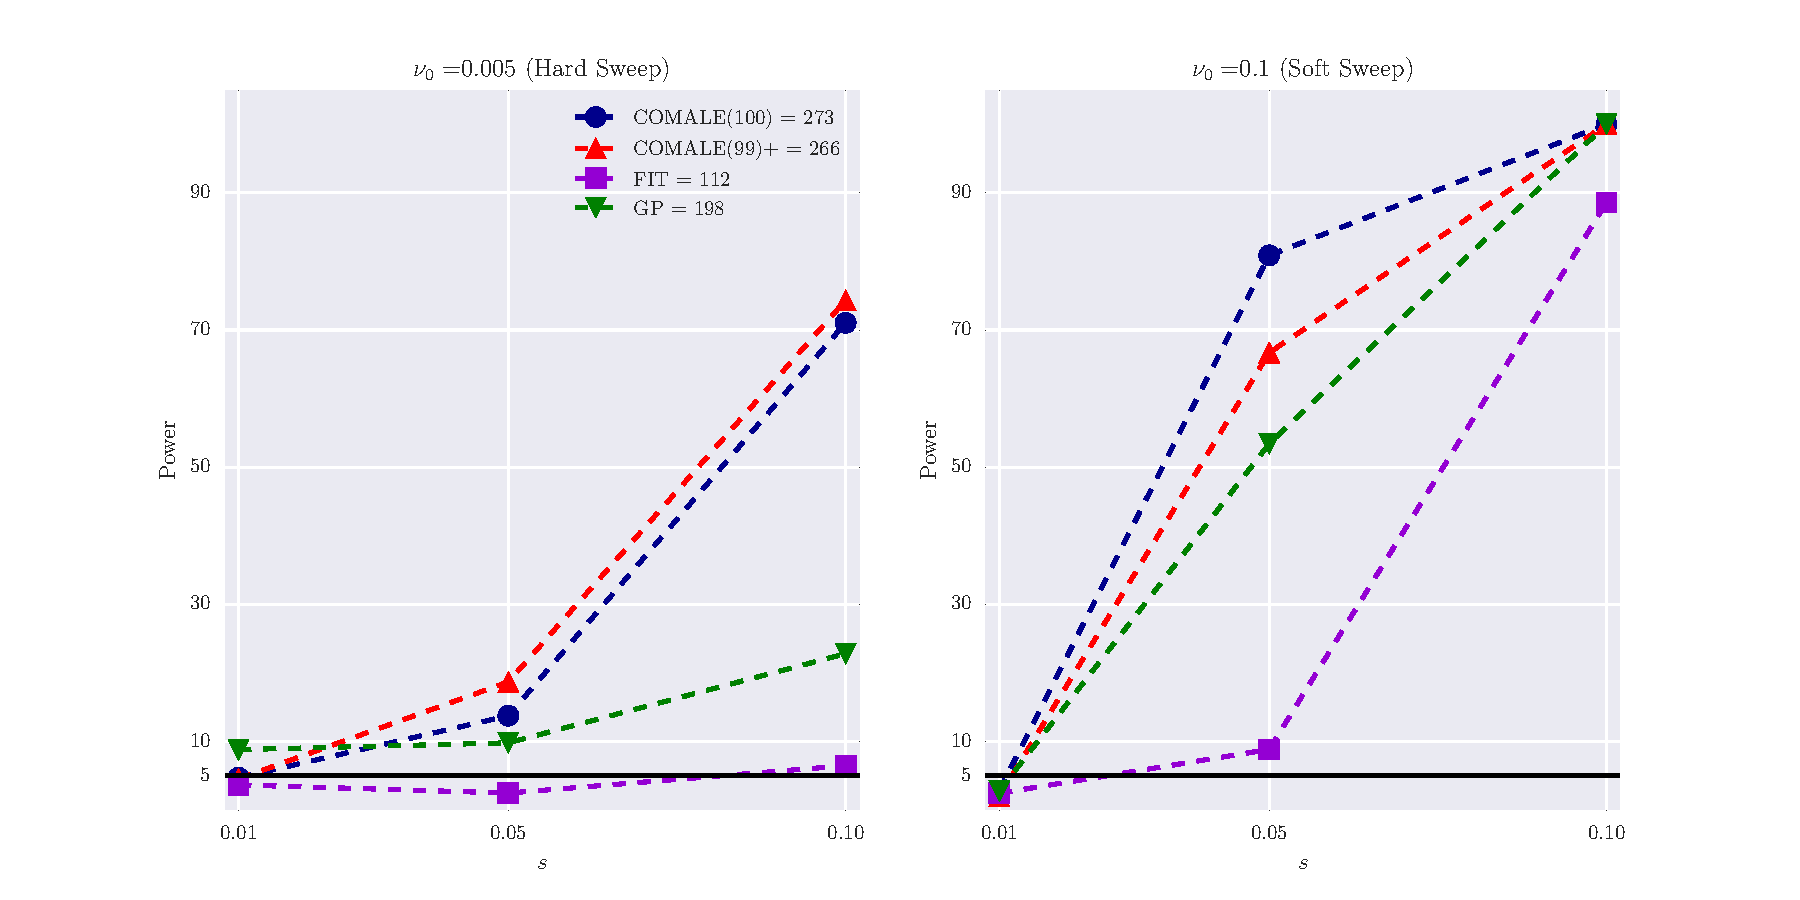
\includegraphics[width=\textwidth]{power.pdf}
	\caption{ {\bf Power calculations for detection of selection.}\\
          Detection power for \comale ($\Hc$), Frequency Increment
          Test (FIT), Gaussian Process (GP), and CMH under hard (A-C)
          and soft sweep (D-F) scenarios. $\lambda$, $s$ denote the
          mean coverage and selection coefficient, respectively.
          Orange hexagons represent the performance of \comale\ when
          the maximum of the single-locus statistic is used to make a
          decision for the genomic region, while the red circle
          corresponds to the performance of \comale\ when single locus
          statistics are averaged over the region.  The $y$-axis
          measures power -- sensitivity with false positive rate FPR
          $\le 0.05$ -- for $2,000$ simulations with $N=1,000$,
          $L=50$Kbp. The horizontal line reflects the power of a
          random classifier.  In all simulations, 3 replicates are
          evolved and sampled at generations
          $\Tc=\{0,10,20,30,40,50\}$.}
           \label{fig:power}
\end{figure}

\begin{figure}[H]
	\centering
	\includegraphics[width=0.75\textwidth]{{runTime.pdf}}
	\caption{{\bf Running time.}\\ Box plots of running time per
          variant (CPU-secs.) of \comale ($\Hc$), CMH, FIT, and
          GP with single, 3, 5, 7, and 10 loci over 1000 simulations
          conducted on a workstation with Intel Core i7
          processor. The average running time for each method is shown
          on the x-axis.
          In all simulations, 3 replicates are evolved and sampled at generations 
          $\Tc=\{0,10,20,30,40,50\}$.}
	\label{fig:runTime}
\end{figure}


\begin{figure}[H]
	\centering
	\includegraphics[trim=.2in 0 .2in 0, 
	clip,width=\textwidth]{{rank100.0}.pdf}
	\caption{{\bf Ranking performance for 100$\times$ coverage.}\\
          Cumulative Distribution Function (CDF) of the distribution
          of the rank of the favored allele in 1000 simulations for
          \comale\ ($H$), Gaussian Process (GP), CMH, and Frequency
          Increment Test (FIT), for different values of selection
          coefficient $s$ and initial carrier frequency. Note that the
          individual variant \comale\ score ($H$) is used to rank
          variants.  The Area Under Curve (AUC) is computed as an overall
          quantitative measure to compare the performance of methods
          for each configuration. In all simulations, 3 replicates with $N=1000$ 
          are evolved and 
          sampled at generations 
          $\Tc=\{0,10,20,30,40,50\}$.}
	\label{fig:rank}
\end{figure}



\begin{figure}[H]
	\centering
\includegraphics[width=0.7\textwidth]{{bias.100}.pdf}
\caption{{\bf Distribution of bias for 100$\times$ coverage.}\\ The
  distribution of bias ($s-\hat{s}$) in estimating selection
  coefficient over 1000 simulations using Gaussian Process (GP) and
  \comale\ ($H$) is shown for a range of choices for the selection
  coefficient $s$ and starting carrier frequency $\nu_0$, when
  coverage $\lambda=100$ (Panels A,B). GP and \comale\ have similar
  variance in estimates of $s$ for soft sweep, while \comale\ provides
  lower variance in hard sweep. Also see \ref{tab:biasdist}. Panels C,D
  show the variance in the estimation of $h$. 
  In all simulations, 3 replicates are evolved and sampled at generations 
  $\Tc=\{0,10,20,30,40,50\}$.}
	\label{fig:bias100}
\end{figure}
\begin{figure}[H]
	\centering
	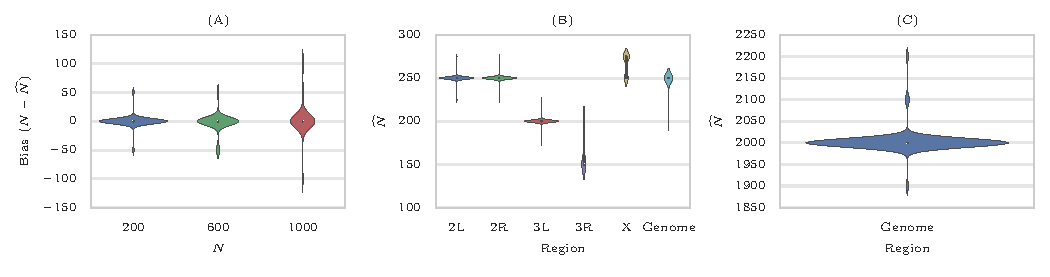
\includegraphics[width=\textwidth]{estimateNMLE.pdf}
	\caption{{\bf Estimating population size.}  (A) Distribution
          of bias in estimating $N$, computed on 1000 neutral
          simulations for each $N\in\{200,600,1000\}$ when $W=10$Mbp and 
          $r=2\times10^{-8}$. (B) 
          Estimates
          of population size for \datadm. For each case, the
          distribution of estimator is computed by 100 bootstrap
          computations using 1000 variants each. The multiple modes
          are an artifact of grid search used to speed up
          computation. (C) Distribution of the population 	size
          estimates on the yeast dataset.  Despite large census
          population size ($10^6-10^7$~\cite{burke2014standing}), this
          dataset exhibits much smaller effective population size
          ($\hN=2000$). }
	\label{fig:estimateNMLE}
\end{figure}

\begin{figure}[H]
	\centering
	\begin{tabular}{c}
		(A)\\
		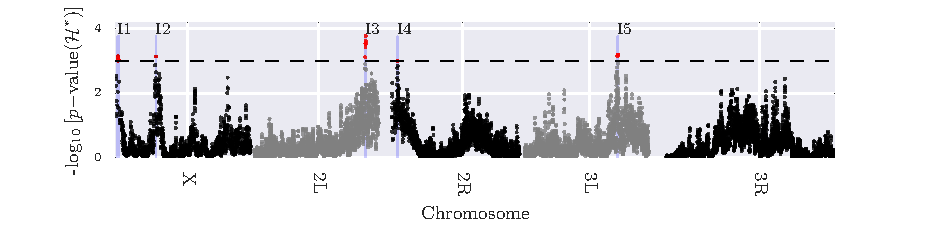
\includegraphics[trim=0.4in 0.in 0.6in 
		0in,clip,width=0.9\textwidth]{man-dmel-region.pdf}\\		
		(B)\\	
		\includegraphics[trim=0.3in 0.in 0.6in 
		.0in,clip,width=0.9\textwidth]{{topVariants.dmel.dir}.pdf}
	\end{tabular}
	\caption{{\bf Scan of \comale\ statistic on \datadm.}
(A)         Manhattan plot of scan for $\Hc^*$ statistic using sliding window of 
size $L=3000$ over the
          genome.  The dashed line represents cutoff for genome-wide
          FDR$\le0.05$, and identifies 5 contiguous intervals, I1-I5, 
          which are shaded in blue. (B) Trajectories of the selected 
          variants within 
          intervals I1-I5.}
	\label{fig:man-dmel-region}
\end{figure}





\begin{figure}[H]
	\centering
	\begin{tabular}{cc}
		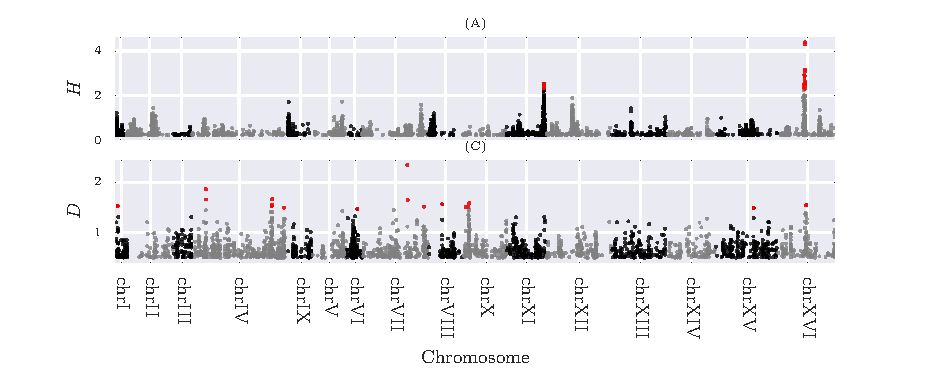
\includegraphics[trim=0.4in 0.in 0.6in 
		0.0in,clip,width=0.65\textwidth]{man-yeast-snp.pdf}&	
		\raisebox{0.2in}{
		\includegraphics[trim=0in 0.in 0in 
		0.0in,clip,width=0.35\textwidth]{{topVariants.yeast}.pdf}}
	\end{tabular}
	\caption{{\bf Single locus analysis of the yeast outcrossing 
	populations.}\\ Manhattan plot 
		of scan single locus \comale\ statistic ($L=1$) for testing directional 
		selection (A) and dominant 
		selection 
		(C).
		The dashed line represents cutoff for  genome-wide FDR$\le0.05$.
		Trajectories of the selected variants are depicted in panels (B) and 
		(D).}
	\label{fig:man-yeast-snp}
\end{figure}


\clearpage
\newpage